\documentclass{article}
\usepackage[utf8]{inputenc}

\title{Real-Time Scheduling Algorithms and battery consumption of mobile devices}
\author{Oscar Rodriguez Arroyo, Raquel Elizondo Barrios, José Daniel Salazar Vargas, Nelson Méndez Montero and Carlos Martín Flores González}

\usepackage{natbib}
\usepackage{graphicx}

\begin{document}

\maketitle

\section{Introduction}

\begin{abstract}
    One of the most increasing areas in application development is real time applications, as time goes by and technology develops more powerful devices the applications are now requested by users as real time applications, extended reality applications, and more complex applications such as on-line banking and more that requires more complex implementations every time. As much as we as users like these new applications and the new possibilities we have with them, there is always a concern regarding this kind of applications in mobile devices: the energy consumption. For this applications to run and perform as expected, a considerable amount of energy is needed, for these applications the constant communication with peers and/or main services is essential, and for that live interaction the device needs to spend more energy than a plain classic application, specifically for jobs that the processor executes periodically to keep the live interaction as expected. There are some approaches for this problem that involve designs of algorithms for scheduling these kind of jobs with the objective of saving energy, or at least spend it wisely. In this paper we discuss some of the algorithms that have been proposed to mitigate this issue and keep the user experience the best possible by using battery energy in a smart way but still guaranteeing a very good performance of real time applications. 
\end{abstract}

\begin{figure}[h!]
\centering
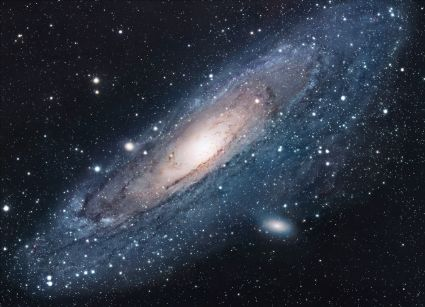
\includegraphics[scale=1.7]{universe.jpg}
\caption{The Universe}
\label{fig:univerise}
\end{figure}

\section{Conclusion}
``I always thought something was fundamentally wrong with the universe'' \citep{adams1995hitchhiker}

\bibliographystyle{plain}
\bibliography{references}
\end{document}
